\chapter{Estruturas de repetição}
Essas estruturas servem para, como o nome já implica, repetir um trecho do algoritmo, seja para garantir que a entrada de dados esteja correta, para refazer uma ação $n$ vezes ou para manter o algoritmo em funcionamento por tempo indeterminado (como no caso de um jogo, onde o jogo só termina quando o usuário pede para sair). Existem três tipos de comandos para repetição, Para, Enquanto e Faça-Enquanto, que são equivalentes entre si, ou seja, pode ser utilizado o de sua preferência.
\section{Contadas}
A repetição contada pode ser utilizada quando sabe-se a quantidade de vezes que o laço deverá ocorrer. Esta quantidade pode ser informada pelo usuário ao se atribuir o valor para uma variável. O comando mais comum para a repetição contada constitui o ``Para''\\
\begin{lstlisting}
Para <variavel> = <valor_inicial> ate <condicao> em passos de <incremento> faca
    <comandos>
    .
    .
    .
Fim-Para
\end{lstlisting}
Para melhor entender o funcionamento da estrutura um pequeno exercício pode ser feito, deve-se determinar a média aritmética de $n$ números. \textbf{Exemplo:}
\pagebreak
\begin{lstlisting}
n, i: inteiro
soma, nro: real
Leia(n)
Soma = 0
Para i=0 ate i<n em passos de i=i+1 faca
    Leia(nro)
    soma = soma + nro
Fim-Para
Escreva(soma/n)
\end{lstlisting}
Note que de $i = 0$ até $i < n$ existem $n$ repetições de 1 em 1. Por exemplo, de $0$ a $5$ passamos pelos números, $0$, $1$, $2$, $3$ e $4$, totalizando $5$ números.
\section{Repetições com teste no começo}
O teste no começo serve para checar se o bloco de código deve ser executado ou se deve ser pulado, como mostra a Figura \ref{fig:repeteComeco}. 
\begin{figure}[H]
    \centering
    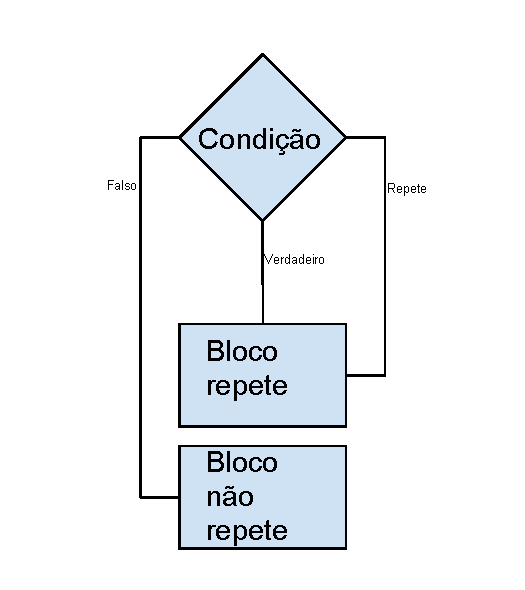
\includegraphics[scale=.75]{repeteComeco.pdf}
    \caption{Fluxograma repetição com teste no começo}
    \label{fig:repeteComeco}
\end{figure}
Pode ser utilizado com a estrutura anterior (Para ... até ... em passos de ...), porém mais comumente utilizado com uma nova estrutura, o Enquanto: \\
\textbf{Estrutura da repetição com teste no começo} \\
\begin{lstlisting}
<variavel> = <valor_inicial>
Enquanto <condicao> faca
    <incremento>
    <comandos>
Fim-Enquanto
\end{lstlisting}
Note que nesta estrutura deve-se inicializar a variável fora do comando da repetição, assim como o incremento fica entre os comandos do bloco e não na repetição em si. Vamos montar o algoritmo para calcular $n!$ (fatorial). \\
Ideia do algoritmo:
\begin{lstlisting}
    Decalaracao de variaveis
    Leia(n)
    Calcula(n!)
    Mostra(n!)
\end{lstlisting}
Já se sabe como declarar, ler e mostrar valores, o calculo de n! se dará por repetição:
\begin{lstlisting}
    fat = 1
    i = 2
    Enquanto (i <= n) faca
        fat = fat*i
        i = i+1
    FimEnquanto
\end{lstlisting}
Para garantir o funcionamento pode-se utilizar o teste de mesa na Tabela \ref{tab:testefatorial}, começando com $n = 5$, por exemplo:
\begin{table}[!h]
    \centering
    \caption{Teste de mesa para o fatorial de 5}
    \label{tab:testefatorial}
    \begin{tabular}{ccccc} \hline \hline
    n & i & (i\textless=n) & fat & saida               \\ \hline
    5 & 2 & Sim            & 2   &                     \\
    5 & 3 & Sim            & 6   &                     \\
    5 & 4 & Sim            & 24  &                     \\
    5 & 5 & Sim            & 120 &                     \\
    5 & 6 & Nao            & -   & Fatorial de 5 é 120 \\ \hline \hline
    \end{tabular}
    \end{table}
\section{Repetições com teste no fim}
Esta última estrutura serve para checar se o bloco de código deve continuar a ser executado, portanto, sempre rodará pelo menos uma vez, já que o teste só aparece ao fim do bloco, exemplificado pela Figura \ref{fig:repeteFim}.
\begin{figure}[H]
    \centering
    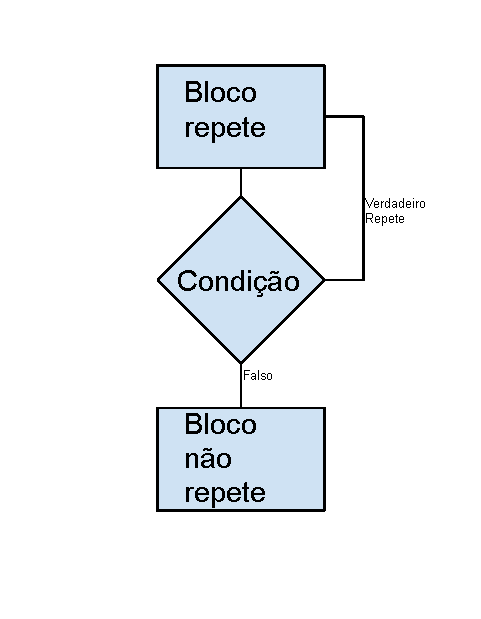
\includegraphics[scale=.75]{repeteFim.pdf}
    \caption{Fluxograma repetição com teste no fim}
    \label{fig:repeteFim}
\end{figure}
\textbf{Sua estrutura segue abaixo:}
\begin{lstlisting}
    <variavel> = <valor_inicial>
    Faca
        <incremento>
        <comandos>
    Enquanto <condicao>
\end{lstlisting}
Da mesma forma que o anterior o incremento deve ser colocado junto aos comandos do bloco. Para exemplo será feito um algoritmo que calcula a soma de valores até que um valor negativo seja lido.
\begin{lstlisting}
    valor: inteiro
    soma: inteiro
    soma = 0
    Faca
        Escreva("Informe um numero")
        Leia(valor)
        soma = soma + valor
    Enquanto (valor >= 0)
    Escreva(soma)
\end{lstlisting}
Para desconsiderar o valor negativo da soma deve-se subtrai-lo ao final da repetição ou adicionar uma condição para não soma-lo durante os comandos da repetição.
\begin{lstlisting}
    valor: inteiro
    soma: inteiro
    soma = 0
    Faca
        Escreva("Informe um numero")
        Leia(valor)
        soma = soma + valor
    Enquanto (valor >= 0)
    soma = soma - valor
    Escreva(soma)
\end{lstlisting}
ou
\begin{lstlisting}
    valor: inteiro
    soma: inteiro
    soma = 0
    Faca
        Escreva("Informe um numero")
        Leia(valor)
        Se (valor >= 0)
            soma = soma + valor
        Fim-Se
    Enquanto (valor >= 0)
    Escreva(soma)
\end{lstlisting}